\documentclass[journal]{vgtc}              % review 

\newcommand{\tool}{{\texttt{FactFlow}}\xspace}
\newcommand{\jieshan}[1]{\textcolor{teal}{#1}}


%% Uncomment one of the lines above depending on where your paper is
%% in the conference process. ``review'' and ``widereview'' are for review
%% submission, ``preprint'' is for pre-publication in an open access repository,
%% and the final version doesn't use a specific qualifier.

%% If you are submitting a paper to a conference for review with a double
%% blind reviewing process, please use one of the ``review'' options and replace the value ``0'' below with your
%% OnlineID. Otherwise, you may safely leave it at ``0''.
\onlineid{1040}

%% In preprint mode you may define your own headline. If not, the default IEEE copyright message will appear in preprint mode.
%\preprinttext{To appear in IEEE Transactions on Visualization and Computer Graphics.}

%% In preprint mode, this adds a link to the version of the paper on IEEEXplore
%% Uncomment this line when you produce a preprint version of the article 
%% after the article receives a DOI for the paper from IEEE
%\ieeedoi{xx.xxxx/TVCG.201x.xxxxxxx}

%% declare the category of your paper, only shown in review mode
\vgtccategory{Research}

%% please declare the paper type of your paper to help reviewers, only shown in review mode
%% choices:
%% * algorithm/technique
%% * application/design study
%% * evaluation
%% * system
%% * theory/model
\vgtcpapertype{application/design study}

%% Paper title.
\title{\tool: Automatic Fact Sheet Generation and Customization from Tabular Dataset via AI Chain Design \& Implementation}

%% Author ORCID IDs should be specified using \authororcid like below inside
%% of the \author command. ORCID IDs can be registered at https://orcid.org/.
%% Include only the 16-digit dashed ID.
\author{%
  Minh Duc Vu, Jieshan Chen, Zhenchang Xing, Qinghua Lu, Xiwei Xu, and Qian Fu
}

\authorfooter{
  %% insert punctuation at end of each item
  \item
  	Minh Duc Vu, Jieshan Chen, Zhenchang Xing, Qinghua Lu, Xiwei Xu, and Qian Fu are with CSIRO's Data61.
  	E-mail: firstname.lastname@data61.csiro.au
  \item
  	Zhenchang Xing is also with Australian National University.
  \item
        Jieshan Chen is the corresponding author.
}

%% Abstract section.
\abstract{%
With the proliferation of data across various domains, there is a critical demand for tools that enable non-experts to derive meaningful insights without deep data analysis skills. To address this need, existing automatic fact sheet generation tools offer heuristic-based solutions to extract facts and generate stories. However, they inadequately grasp the semantics of data and struggle to generate narratives that fully capture the semantics of the dataset or align the fact sheet with specific user needs. Addressing these shortcomings, this paper introduces \tool, a novel tool designed for the automatic generation and customisation of fact sheets. \tool applies the concept of collaborative AI workers to transform raw tabular dataset into comprehensive, visually compelling fact sheets. We define effective taxonomy to profile AI worker for specialised tasks. Furthermore, \tool empowers users to refine these fact sheets through intuitive natural language commands, ensuring the final outputs align closely with individual preferences and requirements. Our user evaluation with 18 participants confirms that \tool not only surpasses state-of-the-art baselines in automated fact sheet production but also provides a positive user experience during customization tasks.
}

%% Keywords that describe your work. Will show as 'Index Terms' in journal
%% please capitalize first letter and insert punctuation after last keyword
\keywords{Fact sheet, infographic, visualisation, visual storytelling, data story, automated design}

%% A teaser figure can be included as follows
\teaser{
  \centering
  \includegraphics[width=\linewidth]{figs/teaser.png}
\caption{%
We demonstrate \tool's functionality using the Tourism dataset. \tool first processes the dataset and the user's initial ideas to automatically generate a fact sheet. Users can then dynamically modify the fact sheet through natural language requests, prompting \tool to generate new content and update the fact sheet accordingly.
}
  \label{fig:teaser}
}

%% Uncomment below to disable the manuscript note
%\renewcommand{\manuscriptnotetxt}{}

%% Copyright space is enabled by default as required by guidelines.
%% It is disabled by the 'review' option or via the following command:
%\nocopyrightspace


%%%%%%%%%%%%%%%%%%%%%%%%%%%%%%%%%%%%%%%%%%%%%%%%%%%%%%%%%%%%%%%%
%%%%%%%%%%%%%%%%%%%%%% LOAD PACKAGES %%%%%%%%%%%%%%%%%%%%%%%%%%%
%%%%%%%%%%%%%%%%%%%%%%%%%%%%%%%%%%%%%%%%%%%%%%%%%%%%%%%%%%%%%%%%

%% Tell graphicx where to find files for figures when calling \includegraphics.
%% Note that due to the \DeclareGraphicsExtensions{} call it is no longer necessary
%% to provide the the path and extension of a graphics file:
%% \includegraphics{diamondrule} is completely sufficient.
\graphicspath{{figs/}{figures/}{pictures/}{images/}{./}} % where to search for the images

%% Only used in the template examples. You can remove these lines.
\usepackage{tabu}                      % only used for the table example
\usepackage{booktabs}                  % only used for the table example
\usepackage{lipsum}                    % used to generate placeholder text
\usepackage{mwe}                       % used to generate placeholder figures
\usepackage{amsmath} 
\usepackage{algorithm}
\usepackage{algpseudocode}
\usepackage{graphicx}
%% We encourage the use of mathptmx for consistent usage of times font
\usepackage{mdframed}
%% throughout the proceedings. However, if you encounter conflicts
%% with other math-related packages, you may want to disable it.
\usepackage{mathptmx}                  % use matching math font
\usepackage{array}
\usepackage{booktabs}
\usepackage{longtable}
\usepackage{appendix}


\begin{document}

%%%%%%%%%%%%%%%%%%%%%%%%%%%%%%%%%%%%%%%%%%%%%%%%%%%%%%%%%%%%%%%%
%%%%%%%%%%%%%%%%%%%%%% START OF THE PAPER %%%%%%%%%%%%%%%%%%%%%%
%%%%%%%%%%%%%%%%%%%%%%%%%%%%%%%%%%%%%%%%%%%%%%%%%%%%%%%%%%%%%%%%

%% The ``\maketitle'' command must be the first command after the
%% ``\begin{document}'' command. It prepares and prints the title block.
%% the only exception to this rule is the \firstsection command

Stochastic systems have been used extensively in several areas including  verification~\cite{FKNP11}, learning theory~\cite{AJKS21}, epidemic processes~\cite{Lef81} to name a few. Several real-world systems however do not work with a centralised control. Therefore, modelling using stochastic systems with multiple agents makes for more faithful abstractions of such systems without a centralised control. Some examples of fields in which multi-agents stochastic modelling include cyber physical systems~\cite{SEC16}, distributed and probabilistic computer programs~\cite{dAHJ01}, probabilistic planning~\cite{TKI10}. In such cases, the problem of reasoning about multiple agents with several, often times orthogonal objectives, becomes important. % However, for situations that are modelled as graph games, Nash equilibria come with its own down-sides and therefore several notions of equilibria have emerged in turn-based games on graphs to circumvent the problems posed by the natural definitions of Nash equilibira, like subgame-perfect equilibira, Stackleberg-equilibria. 
For multi-agent systems modelled with stochasticity on the underlying arena, a fundamental question to ask is the existence or finding of an equilibrium.
The most popular equilibria in literature are Nash equilibria~\cite{Nas50}. However, those come with their own downsides. The computational complexity for studying Nash equilibria over multi-agent systems is prohibitively expensive, and even undecidable in the general case, where systems have $10$ or more players~\cite{UW11}. 
Further, even if Nash equilibria could be computed efficiently, they do not faithfully model the agents in real world settings
%as each agent might perceive risk differently. With randomness arising from both the strategies of other agents, as well as the underlying model of the system, this might mean that risk-averse or risk-loving agents might have an incentive to deviate since their perceived values of outcome is different from expected value of the game.
since they do not consider their tolerance or averseness to risk.

Let us consider a $1$-player game where a protagonist is proposed two options: (a) earning \$1; (b) playing a lottery in which, with probability $\frac{1}{40}$, she gets \$40, and with probability $\frac{39}{40}$, she does not earn anything.
Classically, rational strategies would be maximising the expected payoff. From this perspective, both options yield an expected payoff of \$1, making them equivalent.
This approach is particularly justified when the game represents a scenario that can be repeated many times: the law of large numbers ensures that, in the long run, the average payoff will converge to the expected payoff. However, when the game is played only once, the protagonist may prioritise immediate needs. If she urgently requires \$1, the guaranteed option (a) becomes preferable.

Conversely, if she is a risk-taker or finds herself in a situation where only the \$40 can make a significant difference, she may prefer the high-risk option (b).
Although this choice might appear irrational, it mirrors the behaviour of millions of people who participate everyday in games with a negative expected payoff, driven by the allure of a potentially life-changing win, and generating an annual turnover of USD 536 billions~\cite{GamblingNewspaper23} for the gambling industry.
That industry, on the other hand, operates on a large scale where expected payoff becomes the key metric. 
This contrast underscores the importance of alternative measures to expected payoff that account for each agent's risk tolerance.%, offering a more nuanced understanding of decision-making in uncertain scenarios.

%We thus have an example of a two-player interaction, with apparently zero-sum payoffs, but where both players express a preference for the same option, because the context gives them a different tolerance to risk: this paradox underscores the importance of alternative measures to expected payoff that account for an agent's risk tolerance, offering a more nuanced understanding of decision-making in uncertain scenarios.
% This contrast underscores the relevance of generalising the notion of Nash equilibria: in a multi-agent system, the agents may have diverging perception of which risks can be taken.
% It makes sense, then, to study \emph{risk-sensitive equilibria}, in which players do not necessarily maximise their expected payoff, but their perception of what their payoff will be according to different risk measures.\leon{I'm actually not satisfied with this, I will modify it and move it.}


% Classically, we consider that a rational strategy would consist in maximising the expected payoff: from that perspective, the two choices are equivalent.
% Such an approach is justified especially when the game models a situation that can be repeated a large number of times, in which case the law of large numbers guarantees that the average payoff converges to the expected payoff.
% But when the game models a situation that is played only once, the protagonist may consider that she really needs her euro, and that the possibility of earning 40\$ is too unlikely to be taken into account: she would then have a justifiable preference for the option (a).
% On the contrary, if she is more of a gambler, or if she finds herself in a desperate situation in which only earning those 40\$ could save her, she could go all out and express a strict preference for option (b)\footnote{Even though this case seems more irrational, it explain why millions of people play everyday games in which they know that their expected payoff is negative.
% On the other side, the companies with whom they interact repeat the experience often enough to consider expected payoff as the relevant measure --- generating a yearly turnover of 536 billions of US\$.}.
% Hence the relevance of alternatives to expected payoff, that take into account the tolerance of the agent to risk.

\subparagraph*{Risk Measures.}
A \emph{risk measure} captures the perception that a player has of what their payoff will be. In that sense, they generalise the notion of expected payoff.
Various risk measures exist in the literature, and have been used extensively in the field of economics and finance. 
Some of these risk measures include expected shortfall (ES), value at risk (VaR)~\cite{Aue18}, variance~\cite{Bra99}, entropic risk measure (ER)~\cite{FS02}. 

%However, since the introduction of the characteristic of risk measure called \emph{coherence}~\cite{ADJH99}, it was expected that a ``good'' a risk measure must be coherent. A risk measure is coherent if it is monotonic, homogeneous, translational-invariance, and sub-additive.
%This automatically weeds out several of the above risk measures listed above like  Value at Risk or variance as a risk measure. 
A lot of work has been done in considering these risk measures over MDPs which use variance (along with mean) as a risk-measure~\cite{FK89, PSB22,MT11}, ES~\cite{RRS15,KM18,Meg22} (also referred to as conditional value at risk (CVaR), average value at risk (AVaR), expected tail loss (ETL), and superquantile in literature) and ER~\cite{HM72,BR14,BCMP24}. % have also been studied. 
Studying the entropic risk measure in MDPs appears more practical compared to expected shortfall  or using variance-penalised risk-measures. This impracticability of ES and variance-penalised measure in particular is due to the intractable exponential memory~\cite{HK15} and time required to compute optimal strategies~\cite{PSB22}, even for the one agent system of Markov decision processes (MDPs). On the other hand, when the risk measure used is ER, players have optimal positional strategies in MDPs~\cite{How72}, which makes it a prime candidate for consideration in multi-agent settings.

\subparagraph*{Entropic Risk Measure.}
The entropic risk measure is computed by assigning to each agent a risk parameter, i.e., a value $\rho \in \Rb$.
%Based on this risk parameter $\rho$, this measure first computes the expectation of the exponential function of the random variable and then re-normalises this.  
The entropic risk measure of a random variable $X$ is then defined as
$\re_\rho[X] = -\frac{1}{\rho} \log_e \left( \Eb \left[ e^{-\rho X}\right] \right)$. 
%For computational reasons, instead of the Euler's constant $e$, we use different bases sometimes.
If the risk parameter $\rho$ is positive, then more weight will be given to the bad payoffs: the corresponding player can then be considered as risk-averse.
Conversely, players with a negative $\rho$ are more risk-loving.
When $\rho$ tends to $0$, the entropic risk measure converges to the classical expectation $\Eb[X]$.

The game depicted by Figure~\ref{fig:example_gamma} extends the lottery example we discussed earlier. 
Black vertices are stochastic, and the circle vertex is controlled by player $\Circle$.
A play can be seen as an infinite sequence of moves of a token along the edges of the graph, starting from $a$: from a stochastic vertex, it takes one of the outgoing edges with the probabilities indicated on those, and from a vertex controlled by the player, she chooses which edge it takes.
The payoff $40$, $0$, or $1$ is obtained when the terminal vertex $t_1$, $t_2$, or $t_3$ is reached, respectively.
If no terminal vertex is reached, then the payoff is $0$.
Taking the red edge corresponds to option (a): then, her risk entropy is always $1$, for every risk parameter $\rho$.
But if she chooses option (b), that is, if she takes the blue edge, her risk entropy is $\re_\rho[\mu_{\circ}] = -\frac{1}{\rho} \log \left( \Eb \left[ e^{-\rho \mu_{\circ}}\right] \right) = -\frac{1}{\rho} \log \left(  e^{-40\rho } + \frac{39}{40} \right)$.
Both cases are illustrated with red and blue curves in \cref{fig:example_plot}.
The curves cross at abscissa $\rho = 0$, where the entropic risk measure corresponds to the expectation. Note that other strategies are possible if \emph{randomisation} is allowed---the player could, for example, toss a coin and participate in the lottery if the outcome is heads. The perceived reward of randomising between outermost red and blue edges are illustrated in the intermediate cases with mixtures of red and blue in \cref{fig:example_plot}.

%For this example, we  replace Euler's constant $e$ with instead the constant $2$, which makes $\re_\rho[X] = -\frac{1}{\rho} \log_2 \left( \Eb \left[ 2^{-\rho X}\right] \right)$.

%Player $\Circle$ gets the payoff $11$ if she reaches the terminal vertex $t_1$, the payoff $1$ if she reaches $t_2$, the payoff $2$ if she reaches $t_3$, and the payoff $0$ if she reaches none of those terminal states (i.e., if she loops on the vertex $a$ forever).

%If the player's strategy is to choose the red edge, she gets payoff $1$ with probability $1$.
%Therefore, her risk measure is equal to $1$ for every risk parameter $\rho$.

%If her strategy is to choose the blue edge going to $c$, then she gets the payoff $11$ with probability $\frac{1}{10}$, and $1$ with probability $\frac{9}{10}$.
%Thus her risk entropy is
%$\re_\rho[\mu_{\circ}] = \frac{1}{\rho} \log_2\left(\frac{1}{3} 2^{-4\rho} + \frac{2}{3} 2^{-1\rho}\right)$.
 
\begin{figure}[h] 
			\centering
            \begin{subfigure}[t]{0.4\textwidth}
			\begin{tikzpicture}[->,>=latex,shorten >=1pt, initial text={}, scale=1, every node/.style={scale=1}]
				\node[initial left, stoch] (a) at (0, 0) {$a$};
				\node[state] (b) at (1.5, 0) {$b$};
                \node[stoch] (c) at (2.5, 1) {$c$};
                \node (t1) at (4, 2) {$t_1:~\stack{\circ}{40}$};
                \node (t2) at (4, 0) {$t_2:~\stack{\circ}{0}$};
                \node (t3) at (3, -1) {$t_3:~\stack{\circ}{1}$};
                \path (a) edge[loop above] node[above] {$\frac{1}{2}$} (a);
				\path (a) edge node[above] {$\frac{1}{2}$} (b);
                \path (b) edge[blue, thick] (c);
                \path (b) edge[red, thick] (t3);
				\path (c) edge node[above] {$\frac{1}{40}$} (t1);
				\path (c) edge node[below] {$\frac{39}{40}$} (t2);
			\end{tikzpicture}
			\caption{A stochastic MDP}
			\label{fig:example_gamma}
            \end{subfigure}
            \begin{subfigure}[t]{0.55\textwidth}
			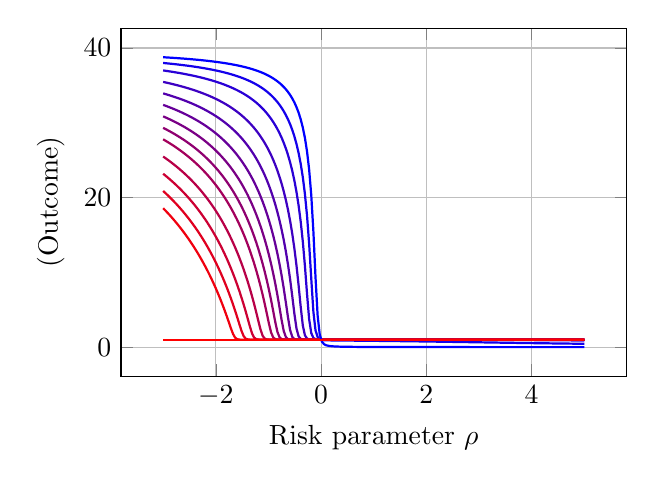
\begin{tikzpicture}
              \begin{axis}[
                xlabel={Risk parameter $\rho$},
                ylabel={$\re(\text{Outcome})$},
                domain=-3:5,
                samples=200,
                    width=8cm,
                   height=6cm,
                grid=major,
                ]
                \addplot [
                  red!8!blue,
                  thick
                ]
                {-1/x * log2((9/10)*e^(-1*x) + (1/400) * e^(-40*x) + (39/400))/log2(e)};
                \addplot [
                  red!16!blue,
                  thick
                ]
                {-1/x * log2((199/200)*e^(-1*x) + (1/8000) * e^(-40*x) + (39/8000))/log2(e)};
                \addplot [
                  red!24!blue,
                  thick
                ]
                {-1/x * log2((19999/20000)*e^(-1*x) + (1/800000) * e^(-40*x) + (39/800000))/log2(e)};
                \addplot [
                  red!32!blue,
                  thick
                ]
                {-1/x * log2((1999999/2000000)*e^(-1*x) + (1/80000000) * e^(-40*x) + (39/80000000))/log2(e)};
                \addplot [
                  red!40!blue,
                  thick
                ]
                {-1/x * log2((199999999/200000000)*e^(-1*x) + (1/8000000000) * e^(-40*x) + (39/8000000000))/log2(e)};
                \addplot [
                  red!48!blue,
                  thick
                ]
                {-1/x * log2((19999999999/20000000000)*e^(-1*x) + (1/800000000000) * e^(-40*x) + (39/800000000000))/log2(e)};
                \addplot [
                  red!56!blue,
                  thick
                ]
                {-1/x * log2((1999999999999/2000000000000)*e^(-1*x) + (1/80000000000000) * e^(-40*x) + (39/80000000000000))/log2(e)};
                \addplot [
                  red!64!blue,
                  thick
                ]
                {-1/x * log2((199999999999999/200000000000000)*e^(-1*x) + (1/8000000000000000) * e^(-40*x) + (39/8000000000000000))/log2(e)};
                \addplot [
                  red!72!blue,
                  thick
                ]
                {-1/x * log2((199999999999999999/200000000000000000)*e^(-1*x) + (1/8000000000000000000) * e^(-40*x) + (39/8000000000000000000))/log2(e)};
                \addplot [
                  red!80!blue,
                  thick
                ]
                {-1/x * log2((199999999999999999999/200000000000000000000)*e^(-1*x) + (1/8000000000000000000000) * e^(-40*x) + (39/8000000000000000000000))/log2(e)};
                \addplot [
                  red!88!blue,
                  thick
                ]
                {-1/x * log2((199999999999999999999999/200000000000000000000000)*e^(-1*x) + (1/8000000000000000000000000) * e^(-40*x) + (39/8000000000000000000000000))/log2(e)};
                \addplot [
                  red!94!blue,
                  thick
                ]
                {-1/x * log2((199999999999999999999999999/200000000000000000000000000)*e^(-1*x) + (1/8000000000000000000000000000) * e^(-40*x) + (39/8000000000000000000000000000))/log2(e)};
                \addplot [
                  blue,
                  thick
                ]
                {-1/x * log2((1/40) * e^(-40*x) + (39/40))/log2(e)};
                \addplot [
                  red,
                  thick
                ]
                {+1};
              \end{axis}
            \end{tikzpicture}
			\caption{Each curve represents the perceived reward of a player choosing only blue strategy, only red, or  randomising between both strategies. The percieved payoff for a player with risk parameter $\rho \in (-3,5)$ for these strategies are represented.}
			\label{fig:example_plot}
            \end{subfigure}
        \caption{Entropic risk measure}\label{fig:example_re}
\end{figure}
%\end{example}
Unfortunately, even for two player zero-sum stochastic games with total-reward objectives (payoff is the sum of the rewards seen along the way), computing optimal strategies can only be done in $\PSPACE$, when the base $e$ is replaced by an algebraic number; and if $e$ is the base of the exponent, then it is decidable only subject to Shanuel's conjecture~\cite{BCMP24}. % and inputs where the risk is computed using ER. 
Solving the two-player zero-sum case is a specific case of finding equilibria in two-agent systems where the payoffs of the two agents are exactly the negation of each others and so are the risk parameters of each of the agents.
Therefore, reasoning about multi-agent systems with ER also has potential to be computationally intractable.%\leon{I'm not sure I understand this sentence}


% \subparagraph*{Equilibria}
% Our example involves only one player.
% However, one might model it with a second player: the company that sells the lottery ticket, and therefore that made the choice of making the game possible.
% Of course, in the real world, companies only enable such games when its expected payoff is positive, that is, when the player's expected payoff is negative; which does not prevent millions of players to participate in such lotteries everyday, generating an annual turnover of USD 536 billion~\cite{h2_gambling_2023}.
% This can be explained by the fact that players are ready to take an important risk there, because they play a small number of times, and their likely loss remains acceptable, while their possible earning would be huge: in other words, players are efficiently modelled by a negative risk parameter.
% On the other hand, the company repeats the game a very large number of times, which is why, from its perspective, the expected payoff is the relevant metric.
% %This contrast underscores the importance of alternative measures to expected payoff that account for an agent's risk tolerance, offering a more nuanced understanding of decision-making in uncertain scenarios.
% This contrast underscores the relevance of generalising the notion of Nash equilibria: in a multi-agent system, the agents may have diverging perception of which risks can be taken.
% It makes sense, then, to study \emph{risk-sensitive equilibria}, in which players do not necessarily maximise their expected payoff, but their perception of what their payoff will be according to different risk measures.\leon{I'm actually not satisfied with this, I will modify it and move it.}



\subparagraph*{Extreme Risk Measure.} We introduce a new risk measure called extreme risk measure (XR) to identify tractable risk parameters. %\leon{Do we actually use that notation?} 
% If they have to choose between two options: (a) one which always gives him an outcome of 1, and the other option (b) that gives him a positive probability $p$ of 100, but  probability $(1-p)$ of -1, he would always chose option (a), 
%
%Let us say in a stochastic system, one agent is tasked with a safety-critical objective and wishes to avoid any positive probability of getting a payoff below some threshold, say $0$.
Consider an agent who wishes to maximise the lowest payoff received with positive probability.
In our example, 
by choosing option (a) her only payoff is $\$1$, whereas by choosing option (b), the payoffs that she receives with positive probability are $\$40$ and $\$0$. 
This agent would choose the option (a) since, then, the lowest reward she gets is $\$1$, instead of $\$0$. This would be her choice regardless of the probabilities or if the lottery amount in option (b) is increased.
%Even when the probabilities are changed for option (b) or if the lottery amount is increased, she would still prefer option (a).
Such agents can be considered ``extreme pessimists'' because
their perceived payoff can be thought of as the minimum among all the possible payoffs.
%We define the perceived reward of an extreme pessimist as the infimum of the payoffs that they get with positive probability. Therefore, extreme pessimists aim to maximise the smallest payoff that they receive with positive probability, and might be willing to deviate to achieve this objective.  
Similarly, one can define ``extreme optimists''  whose perceived reward is the best payoff that can be obtained with positive probability.
In the above scenario, an extreme optimist posed with the same options would choose option (b), no matter how small the probability is of receiving that payoff.

Extreme pessimists can be used to model safety-critical agents, where any positive probability of low reward or failure is unacceptable.
On the other hand, extreme optimists model naturally the opponents of such agents.
In a multiplayer setting, they can be an accurate modelling of agents like hackers in a system, who are happy with a small probability of success, or agents that have the possibility to restart their interactions with the same system, so that as long as there is a non-zero probability of achieving a high reward, they are guaranteed to receive that high reward. %\theju{If at all we discuss motivation here is the space.}





%\begin{example}
% Consider the same example game as in \cref{fig:example_gamma}. Here, the reward that the player perceives in the MDP can perceive on using the red strategy is exactly $2$ since that is the only payoff the player can get with a positive probability.
% However, if using the blue strategy, the perceived reward depends on if the player is an optimist or a pessimist. If the players is a pessimist, then the perceived reward is $4$, and if instead the player is an extreme pessimist, then the perceived reward is $1$.
%\end{example}
% \thejaswini{Introduce with examples some systems that need to be designed where some agent needs sure reward, and agents that some agents are happy with non-zero probability of reward}

%We capture this concept of extreme optimism and pessimism by introducing a new risk measure of pessimistic expectation and optimistic expectation.
\subparagraph*{Our results.}
We consider the problem of finding equilibria in a multiplayer stochastic game, that is, a game in which the payoffs that the players receive depend on the \emph{terminal vertex} that is reached, and in which an infinite play is associated to the zero payoff vector.

Our contributions are four fold. 
Firstly, we consider the problem of finding equilibria where entropic risk measure is used to determine the perceived reward of each player.  Each player has their own risk-sensitivity parameter, and we wish to find an equilibrium where no player has the incentive to deviate and increase their risk measure. We show that, when the rewards are all non-negative, such an equilibrium always exists.
We conjecture that this remains true when rewards can be negative.
Although some equilibria exist, not all equilibria are made the same, with some equilibria being more desirable than the others. One might want to find an equilibrium that maximises the overall social welfare, or want to minimise it for certain agents. A reasonably general setting is providing an interval for the risk measure for each agent and to check if there is an equilibrium satisfying these constraints. We call this problem \emph{constrained existence problem of risk-sensitive equilibria} (RSEs). 
We show (in \cref{sec:ERM}) that this problem is undecidable when the risk parameters of the players are rational values, with undecidability results extending from the constrained existence problem for Nash equilibria in the work of Ummels and Wojtczak~\cite{UW11}. However, we find restrictions on strategies to recover decidability. % for risk-sensitive equilibria in the cases where the risk parameters are finite.
If we restrict the memory requirements of each player, then for (small) finite memory strategies, we can solve the problem by encoding it using the existential theory of reals with exponentiation, giving us decidability subject to Shanuel's conjecture, and $\PSPACE$ algorithms when the base of the exponents are encoded as small algebraic instances, reminiscent of the two-player zero-sum case by Baier et al.~\cite{BCMP24}. 
%(\cref{proposition:Undecidable}).

Secondly, since the general problem is undecidable, and even in restricted cases, we obtain complexities that are $\PSPACE$ or higher, we pivot to searching for a more tractable risk measure that can be used to find equilibria in multi-agent systems. We define extreme risk measure (XR) as a novel risk measure to consider in multi-agent stochastic systems. We show (in \cref{sec:XR}) that our new definition is robust, since it exactly captures the well-studied entropic risk measure when the risk parameters tend to $\pm \infty$.
%This result (\cref{thm:RE=PEorOE}) in turn ensures that our risk measure is a robust definition since it is the limit of a well-studied risk measure. 
We further show the existence of 
such equilibria for games with non-negative rewards. Moreover, there exists a stationary strategy profile that can be algorithmically constructed in polynomial time. We conjecture, again, that this remains true when negative rewards are involved.
One further advantage of XR as a risk measure is that it is indifferent to the exact probabilities of the underlying stochastic model, since it only deals with events that occur with a positive probability and, therefore, can also be used in systems where the underlying probabilities are unknown. 

Thirdly, we show that the constrained existence problem of RSEs is decidable and also $\NP$-complete when the perceived payoff is calculated using XR, where each agent is either an extreme optimist or pessimist. The $\NP$ membership is nontrivial and follows several steps. First, we show that if there is a strategy that satisfies the constraints, then there is a finite abstraction of this strategy. Later, we show that this finite abstraction of the strategy has a polynomial representation. 
With this polynomial representation of the strategy, we show that verifying whether a given polynomially represented strategy is a risk-sensitive equilibrium that satisfies the constraints can also be done in polynomial time. 
Finally, we show that if all players are extreme optimists, this problem is $\PTIME$-complete.%, and provide a polynomial time algorithm for the constrained existence problem.
%\thejaswini{We add to this list by introducing a new risk measure that captures the above situation of extreme optimism and pessimism.}
%\thejaswini{We argue that our definition is robust, since this exactly captures the ERisk measure when the parameters are set to $-\infty$ and $+\infty$}
% \thejaswini{When the parameters are anywhere that are not $\pm\infty$, we show that computing Equilibria where ERisk is the outcome is undecidable. }
% \thejaswini{Argue that however, computational costs of precisely computing RSE for such values for stochastic games are undecidable}
% \thejaswini{This makes our definition the only decidable fragment for finding equilibria with entropic risk as a measure decidable}
\section{Related Works}

\subsection{Data Analysis and Visualisation Tools}

Data analysis and visualization tools have seen significant advancements in recent years. Earlier tools like Excel and R required substantial manual effort and expertise, but there has been a notable shift towards automation. This transformation is driven by research efforts that have progressively automated various aspects of the data analysis process~\cite{wu2021ai4vis}. Initial research focused on providing visualization recommendations from datasets~\cite{cui2019datasite,kim2020gemini,wongsuphasawat2015voyager}, aiding users in the visualization process. Other work improved existing visualizations by focusing on aspects such as visual style searching~\cite{hoque2019searching}, assessing visualizations~\cite{fu2019visualization}, and annotation placement~\cite{bryan2016temporal}. Industrial tools like Tableau and Power BI have begun integrating AI to streamline data management for business applications~\cite{itsnotaboutthecell,nichols_wang_2024}. Although these systems have proven useful for data workers, novice users still face challenges in creating visualizations due to a lack of expertise.

Recent research has shifted towards automatically generating charts from datasets. Data2Vis~\cite{dibia2018data2vis} and VizSmith~\cite{vizsmith} demonstrated the feasibility of generating structured code in Vega-Lite and Python to produce appropriate graphs. Despite these advancements, a common limitation has been the inadequate integration of the human perspective in the outputs. The generated visualizations may not fully align with user intentions, limiting the usability of these systems. NL4DV~\cite{narechania2020nl4dv} addressed this by enabling chart generation based on natural language requests, aligning outputs more closely with user preferences. This capability was further enhanced by NL2Viz~\cite{wu2022nl2viz}, which incorporated program context to better capture user intentions. However, heuristic-based semantic matching in these tools still struggled with linguistic challenges, such as synonyms. For instance, terms like \emph{``yearly''} and \emph{``annual''} were not recognized as equivalent. Recently, LLMs have been applied to data visualization tasks, solving the problem of natural language semantic understanding and accommodating greater flexibility in user input~\cite{chat2vis}. While this research has shown positive results with various prompt techniques, we aim to explore how specialized AI worker definitions can further improve the quality of generated charts.


\subsection{Automatic Story-Telling and Fact Sheet Generations}

In scenarios where isolated visualizations fail to convey complex datasets effectively, narrative visualizations play a crucial role in presenting data with an intuitive and coherent flow, thereby enhancing accessibility for general audiences~\cite{ren2023re}. Narrative visualizations encompass a range of representations, including data videos~\cite{wang2021animated}, data comics, storylines~\cite{liu2013storyflow}, and infographics~\cite{cui2019text}. Early technologies provided platforms for users to manually design story flows. For example, Infonice~\cite{wang2018infonice} assisted users in creating infographics, bridging the gap between data exploration and presentation. Similarly, DataSelfie~\cite{kim2019dataselfie} enabled users to create personalized data visuals. However, these tools required a deep understanding of data and experience in composing data storytelling artifacts, limiting their accessibility to general users.

Recent technological advancements have led to the development of automated storytelling approaches~\cite{chen2023does}, offering a more accessible method for composing storytelling artifacts. These tools capture information from datasets and craft narratives around them. AutoClip~\cite{shi2021autoclips}, for example, automatically generates data videos to showcase fact findings. NewsViews~\cite{gao2014newsviews} provides an automated pipeline that extracts topics and creates corresponding geographic visualizations using contextual information from articles. Focusing on a more concise and data-driven format, recent advancements have also targeted the automated generation of fact sheets. DataShot~\cite{wang2019datashot} was the first tool to automatically generate fact sheets from tabular datasets, focusing on deriving quality facts from the data. However, this approach overlooked the overall story flow due to a lack of semantic relationship identification between different visualizations. Calliope~\cite{shi2020calliope}, an improvement upon DataShot, applied a logic-oriented Monte Carlo tree search algorithm to construct the story from facts. Despite this enhancement, Calliope still faces challenges in creating a seamless narrative across different visualizations due to limited understanding of data semantics. Additionally, previous fact sheet generation approaches did not consider user input and struggled with generating engaging textual components, such as chart titles and descriptions, due to their reliance on template-based methods~\cite{shi2020calliope, wang2019datashot}. Building on this evolving research trajectory, \tool aims to enhance the integration and natural flow of charts with more precise and natural captions.


\begin{figure*}[h]%[tb]% specify a combination of t, b, p, or h for top, bottom, on its own page, or here
  \centering % avoid the use of \begin{center}...\end{center} and use \centering instead (more compact)
  \includegraphics[width=\textwidth]{figs/overview.pdf}
  \caption{%
Workflow of \tool for generating a fact sheet using a global population dataset with columns for Country, Population, and Continent. \tool first prepares the dataset representation, which is then processed by the AI Chain. Each worker in the chain is profiled for specific tasks to generate the fact sheet.
}
  \label{fig:overview}
  \vspace{-4mm}
\end{figure*}

\subsection{Large Language Models for Data Tools}
Recent advancements in generative AI have driven the development of Large Language Models (LLMs), designed to understand natural language and generate human-like responses. Through prompt engineering techniques~\cite{min2022rethinking}, LLMs have improved the accuracy of heuristic-based solutions while reducing the need for extensive data and complex model training. Research on the applicability of LLMs spans various fields, from healthcare~\cite{cascella2023evaluating} and finance~\cite{wu2023bloomberggpt} to IT sectors like testing~\cite{deng2023pentestgpt}, automation~\cite{schwartz2023enhancing}, and smart devices~\cite{king2023get}. However, LLMs struggle with complex multi-step tasks, necessitating further research to enhance their usability. To address this, Wu et al. introduced AI chains~\cite{wu2022ai}, which break down complex tasks into manageable subtasks, each handled by a specific prompt. PromptSapper builds on this concept by defining the roles and collaboration of workers within the chain~\cite{cheng2024prompt}.

In the domain of data tools, pioneering research has explored the capabilities of LLMs in generating visualizations and aiding other visualization-related tasks. LLM4Vis, for instance, conducted experiments using a ChatGPT-based approach for visualization recommendations~\cite{wang2023llm4vis}, demonstrating the model's applicability for data tasks. Additionally, Chat2VIS~\cite{chat2vis} conducted a comparative study on the abilities of ChatGPT, Codex, and GPT-3 in rendering single visualizations from language queries. Other studies have also explored enhancing user interaction with visualizations by integrating LLMs to develop chatbot assistants for datasets~\cite{kavaz2023chatbot}. Recently, ChartGPT~\cite{tian2024chartgpt} performed fine-tuning of LLMs on a specialized dataset of visualizations to generate accurate and expressive charts from abstract natural language inputs. Additionally, DataTales~\cite{sultanum2023datatales} utilized LLMs' natural language capabilities to generate textual narratives accompanying charts in data-driven articles. This research has paved the way for advanced LLM applications in creating robust, user-centric data tools. Building on this, \tool adopts a holistic approach, leveraging LLMs to generate complete fact sheets from tabular datasets. Our goal is to apply AI chain techniques to tackle complex data tasks and validate their feasibility.

\section{System Design}

We introduce \tool, an automated fact sheet generation system, as shown in \cref{fig:overview}. \tool applies the concept of an AI chain to generate fact sheets based on data and user requests. Users can further customize the fact sheet, such as by adding new facts or rearranging content. In this section, we first highlight the AI worker profiling and workflow, followed by a detailed description of the fact sheet generation process. Lastly, we present the \tool’s interface for generating and customizing fact sheets.

\subsection{AI Worker Profiling \& Workflow}
\label{sec:agent}

While simple prompting techniques can effectively handle straightforward, isolated tasks, such as visualization code generation, they face challenges when applied to more complex, integrated tasks. First, LLMs often lack domain-specific knowledge, which can result in outputs that do not meet the nuanced requirements of specialized tasks. Second, providing an abstract task without thorough step-by-step planning can disrupt the overall process, as LLMs may fail to propose the necessary sequence of actions to achieve the desired outcome. Finally, there can be incompatibilities between subtasks, where outputs from one stage may not align with the inputs required by the next, leading to pipeline failures and hindering task completion. To address these issues, we adopted the AI chain approach for generating fact sheets from tabular datasets. This approach leverages specialized AI workers, known as agents, each designed to handle specific subtasks more efficiently. These agents possess unique knowledge and capabilities tailored to their specific tasks, allowing them to focus on their assigned roles with greater precision, thereby improving the overall quality of the output. We define each worker with the following attributes:


\textit{Overall Goal \& Specific Role.} To simulate the positive impact on work outcomes and productivity, we provide overall goals before detailing individual tasks, mirroring real-world scenarios~\cite{barrick2013theory}. The workers share common objectives while working on specific parts of the pipeline, stimulating goal-directed behaviors~\cite{sioutis2006agent}. The specific role of each worker in the AI chain is then defined to achieve the overall objective.

\textit{Persona.} Persona refers to how each individual behaves and thinks~\cite{10.1145/3613904.3642406}, which has been shown to be crucial in optimizing the effectiveness of AI workers~\cite{10.1145/3640794.3665887}. While LLMs do not have a default persona, we manually define the persona of each worker, including the characteristic traits, motivation, and expertise necessary for successfully completing assigned tasks. For example, the Fact Composer is specified to be creative and analytical, while the Data Extractor is meticulous and knowledgeable. Further details of the AI workers we defined can be found in Section~\ref{sec:factideas}.


\textit{Input \& Output.} We provide a list of input and output variables with their descriptions, formats, and data types that the agent receives or returns. This improves the reliability of the overall pipeline. Additionally, we include few-shot examples following this input and output format, which further enhances the reliability and alignment of the output~\cite{song2023llm}.

\textit{Knowledge Base.} This refers to specialized domain knowledge that supplements the general capabilities of LLMs. For each task assigned to a worker, we compile and refine relevant datasets and prior research to build a tailored Knowledge Base. This allows the agent to perform optimally in its specialized task, avoiding the hallucination effects of LLMs when dealing with complex user requests~\cite{martino2023knowledge}.

\textit{Instructions.} Research has shown the importance of sub-step guidance over abstract instruction for task performance accuracy~\cite{madaan2022language}. Therefore, we include step-by-step procedures that each worker follows to achieve its objectives.

Our AI workers utilize a decentralized communication model, where interaction occurs directly between related agents~\cite{cheng2024prompt}. Upon completing a task, an agent forwards its output to the next designated agent in the workflow. To maintain consistency, all input and output data are standardized in JSON format, adhering to REST API protocols. For transmitting object files, such as images or data files, these are stored as block objects, with the directory path provided for file retrieval. 


\subsection{Fact Sheet Generation}

Upon receiving the dataset and, optionally, a user request, the fact sheet generation process begins. \tool first analyzes the dataset to create a dataset representation and then utilizes the AI workers described in \cref{sec:factideas} to generate the fact sheet structure and visual components. Following this, we arrange the fact sheet contents on the canvas and export the initial fact sheet.


\subsubsection{Dataset Representation}
\label{sec:anomysation}

Given that LLMs process input as textual prompts, our goal is to identify the optimal method for capturing and conveying the essential details of the input dataset. Traditional approaches often involve feeding the entire dataset to the LLM, but this method faces significant limitations. Firstly, LLMs have token constraints, making it impractical to handle large datasets. Additionally, directly exposing the entire dataset can compromise privacy and intellectual property. Therefore, our approach focuses on incorporating sufficient dataset information into the prompts to guide LLMs in making accurate decisions without directly providing the dataset. We achieve this by presenting the dataset using SQL table creation commands, column statistics, and example rows. An example of dataset representation for the Global Population dataset with 3 columns (Country, Population, Continent) is shown in \cref{fig:overview}.

\textit{SQL Table Creation Command.} To capture the table name and column names along with their corresponding data types, we use SQL table creation command syntax. This approach also aids our AI workers in better formulating and generating SQL query syntax in subsequent processes. 

\textit{Column Statistics.} For each column, we generate statistics that summarize the values it contains. For numerical columns, this includes the maximum, minimum, median, average, and the 25th and 75th percentiles. For string columns, we count the number of unique values and identify the top five most frequent occurrences. These statistics provide LLMs with a comprehensive overview of the data range.

\textit{Anonymized Data Examples.} We include anonymized sample rows from the dataset to help LLMs understand the expected data values in each column. The number of rows presented depends on the token limits, with more columns requiring more tokens. Given that the input data may contain private information or intellectual property, anonymization is crucial to protect the confidentiality of the data~\cite{lin2024promptcrypt}. We employ a format-preserving encryption technique that maintains semantic integrity, preserving the semantic meaning and ordinal relationships of the data during anonymization. This allows LLMs to comprehend the underlying data structure without directly accessing the original dataset. The anonymization process involves classifying each column by its data type—nominal, ordinal, discrete, or continuous—and applying a tailored anonymization method.

\begin{itemize}

\item \textit{Nominal values} are qualitative and lack a specific order or comparability. To anonymize these values while preserving meaning, we substitute them with semantically equivalent terms. For instance, if the column refers to country names, ``France'' might be replaced by ``Italy.'' We use the column's entity type to guide this substitution, generating random values for each entity type and mapping them to unique values in the data.
\item \textit{Ordinal values} have a specific order, and maintaining this order during substitution is crucial to avoid inconsistencies in later analysis. For example, in a letter grading system where grades are A, B, C, D, and F, substituting these grades with random values could lead to confusion, such as when querying how many students received a grade better than C. To prevent this, we first extract all valid values from the dataset and ensure that the anonymized values are selected from this pool.
\item \textit{Discrete numerical values} are anonymized using a mathematical transformation that maintains the ordinal relationships between values. For example, if the original values are integers representing counts, the transformed values will still reflect the same relative magnitudes, ensuring consistency in any subsequent analysis.
\item \textit{Continuous values} such as those found in time series data, are treated with a different approach. We anonymize these by generating new random values within the original range, ensuring that the data remains realistic and usable while masking the exact figures.
\end{itemize}

 
\subsubsection{Fact Sheet Content Generation}
\label{sec:factideas}

After anonymizing the dataset, we feed the data into our AI chain to generate the fact sheet content. Users can provide additional requests in natural language to specify their requirements for the dataset. This feature is particularly useful when users are interested in covering only a specific portion of the dataset rather than the entire dataset. For example, a user may request data within a limited time range or focus on specific columns. This section discusses how each agent handles its tasks in the pipeline.

\textit{Fact Idea Composer.} 
The primary task of this agent is to generate fact ideas from the dataset. To enhance the agent's capability, we incorporated expert knowledge from a prior study that categorizes facts into eleven distinct types such as Distribution, Categorization, Trend and Rank~\cite{wang2019datashot}. Additionally, we conducted a design session with three senior data scientists, providing each with ten distinct datasets and asking them to suggest interesting facts for a fact sheet. We refined these suggestions by removing duplicates and resolving ambiguities, integrating the refined list of fact ideas into the Fact Idea Composer's knowledge base\footnote{\url{https://anonymous.4open.science/r/factflow-public-2BF8/knowledgeBase}}. This ensures that the generated fact ideas align closely with expert expectations and are grounded in the actual data context. The agent is instructed to generate all potential facts and rank them based on relevance and significance, filtering out less important or redundant facts. The Fact Composer Agent employs the self-consistency prompting technique~\cite{cheng2024relic}, using multi-turn communication to ensure output accuracy. The agent's output consists of a list of fact ideas, each categorized by fact type and content.

\textit{Data Extractor.}
Since each fact represents only a portion of the original dataset, \tool involves the Data Extractor to retrieve the data relevant to the fact. This agent receives a fact idea, additional user requests, and the dataset representation to generate an appropriate SQL command to query the original dataset. To improve the accuracy of converting natural language to SQL (NL2SQL), we added into the agent's knowledge base the Spider dataset~\cite{yu-etal-2018-spider}, which is a well-known dataset containing the natural language questions and its corresponding SQL command. Given the challenges LLMs face in code generation, particularly in terms of robustness and accuracy~\cite{yu2023llm}, we apply the Code Generation with Advising and Validation approach~\cite{chen2023seed}. The agent first lists recommendations for code generation, considering data types and required facts. It then generates an executable SQL command to query the data locally. In the validation step, the agent presents the data representation obtained from the initial query, along with the SQL command, to the LLMs to refine any syntactical errors. Upon completion, the agent outputs the filtered dataset relevant to the fact idea.


\textit{Data Visualizer.}  
After filtering the data, each fact idea is presented through a visualization. The Data Visualizer uses the dimensions of the filtered dataset provided by the previous agent to recommend the most appropriate visualisation type and visual encoding channels  To ensure the fact sheet's accessibility to a wide range of users, \tool supports widely recognized visualization types such as line charts, bar charts, scatter plots, pie charts, and area plots. We limit the number of encoded dimensions to three, resulting in a 2D chart with color as the maximum additional encoding. Unlike previous approaches that relied on direct code generation for creating graphs, we implemented a parameter-driven approach. In this method, a function generates different types of visualizations based on input parameters provided by the agent. These parameters may include chart type, data dimensions, axis labels, color schemes, and more. To enhance the Data Visualizer's capability in generating accurate and relevant visualizations, we documented the function’s input and output parameters. This documentation serves as a knowledge base, guiding the agent in appropriately configuring the parameters to produce the desired visual outputs.


\textit{Fact Writer.}
The Fact Writer leverages the processed dataset and visualizations from previous agents to generate factual statements that are well-aligned with the context provided by the charts. Additionally, the agent aims to clarify the underlying rationale of the presented data. While some inquiries related to the data can be directly addressed using the processed data from previous steps, others require a broader knowledge base for comprehensive explanation. Therefore, we instruct the agent to generate questions regarding the causal relationships in the presented data. The Fact Writer uses LLMs to create additional questions that explore the causation effects of external contexts, such as related historical events or geographical information. These questions help explain the key data points highlighted in the chart or explain what the fact implies. For example, if the dataset shows that France is the most visited country for tourism, the agent might ask, \textit{``Why is France the most visited country for tourism?''} to gain deeper insights and present them. This enriched content significantly enhances the viewer's understanding and interpretation of the charts, especially when dealing with complex data that might be unfamiliar to the audience.


\textit{Factsheet Organizer.}
The primary goal of this agent is to structure the fact sheet in the most logical order to enhance the learnability of the presented information. Our fact sheet contains different sections, each presenting a key topic with a list of relevant charts to support the idea. Using the list of facts and generated material from other workers, the Fact Sheet Organizer finds relevancy between facts to form the story flow with several key topics. After that, the agent sorts the list of facts into these topics based on the relevancy and outputs the structure of the fact sheet in JSON format for fact sheet generation.


\begin{algorithm}
\caption{Split Sections Into Columns}
\label{alg:split_sections}
\begin{algorithmic}[1]
\Require A list of $sections$
\Ensure A boolean list for column layout
\Function{split\_columns}{$sections$}
    \State $best\_diff \gets \infty$, $best\_layout \gets \text{None}$
    \For{$perm$ in $\text{permutations}(sections)$}
        \For{$comb$ in $\text{powerset}(\text{range}(1, \text{len}(perm)))$}
            \State $left\_score \gets \text{calculate\_score}(perm[0])$
            \State $right\_score \gets 0$
            \For{$i \gets 1$ \textbf{to} $\text{len}(perm) - 1$}
                \If{$i$ in $comb$}
                    \State $left\_score \gets left\_score + \text{calculate\_score}(perm[i])$
                \Else
                    \State $right\_score \gets right\_score + \text{calculate\_score}(perm[i])$
                \EndIf
            \EndFor
            \State $diff \gets \text{abs}(left\_score - right\_score)$
            \If{$diff < best\_diff$}
                \State $best\_diff \gets diff$, $best\_layout \gets (perm, comb)$
            \EndIf
        \EndFor
    \EndFor
    \State Convert $best\_layout$ to boolean list $result$
    \State \Return $result$
\EndFunction
\end{algorithmic}
\end{algorithm}


\subsubsection{Fact Sheet Layout}
\label{sec:layout}

\begin{figure*}% specify a combination of t, b, p, or h for top, bottom, on its own page, or here
  \centering % avoid the use of \begin{center}...\end{center} and use \centering instead (more compact)
  \includegraphics[width=0.8\linewidth]{figs/customisation.pdf}
  \caption{%
  	Our \tool interface: a) User can upload dataset and provide any additional natural language request to generate the fact sheet b) Based on the initial fact sheet, users can manually add, remove and edit the content, as well as generating a new fact using natural language request.
  }
  \label{fig:customisation}
    \vspace{-4mm}
\end{figure*}

After establishing the structure of the fact sheet, we proceed to design its layout. We advocate for a dual-column layout to enhance readability and minimize eye movement~\cite{shrestha2008eye}. The layout consists of multiple sections within each column, arranged vertically. Our objectives in developing the layout are twofold: 
First, to preserve the original logical order of the sections as outlined in the fact sheet structure, thereby enhancing its storytelling attributes. Second, to achieve a balanced distribution of content between the two columns. This balance not only contributes to the aesthetic appeal of the fact sheet but also ensures content readability. A key challenge is dividing sections into two columns, given the varying sizes of each section due to differing numbers of facts. To address this, we assign a fixed height to each fact and calculate the cumulative height of each section. We then apply an optimization algorithm to distribute sections across the columns, as described in \cref{alg:split_sections}. This algorithm processes an array of section heights in logical order and outputs a boolean array, assigning sections to the left column as ``True'' and to the right column as ``False''. The Introduction section is always placed at the top left, so the first array value is set to ``True'' by default. \tool then uses this layout structure to iteratively assign sections to the columns, generating the complete fact sheet.



\subsection{Fact Sheet Customization} 
\label{sec:customisation}

In developing our automated pipeline for fact sheet generation, we emphasize the synergy between human input and AI automation, aiming to enhance human-AI collaboration with AI as an assistant in various tasks. To support this, we provide an interface that allows users to create and customize AI-generated content within the fact sheet. Users start by uploading their dataset on the Upload page (\cref{fig:customisation}a) and can specify their interests. We also offer two sample datasets for experimentation.

Upon clicking Begin, \tool automates the fact sheet generation and directs users to the Editor page (\cref{fig:customisation}b), where they can dynamically tailor the content to their needs. The interface allows users to add, remove, and rearrange sections according to their preferences. For each visualisation, users can delete, rearrange or move them across sections. \tool supports adding new charts based on natural language request, processing this as new fact ideas through the AI chain to generate corresponding charts and textual content. This new fact will be presented in appropriate section automatically. After customization, users can export the fact sheet as a PDF. The generated content will be stored with the unique ID, where user can further continue to modify the same fact sheet in the future.

\subsection{Implementation}

\begin{figure*}[!h]% specify a combination of t, b, p, or h for top, bottom, on its own page, or here
  \centering
   \label{fig:showcase}
  \begin{subfigure}[t]{0.50\textwidth}
  	\centering
  	\includegraphics[width=\textwidth]{figs/factsheet-1.pdf}
  	\caption{Fact sheet about startup failures after the tide of ``new economics'' in China.}
  	\label{fig:showcase1}
  \end{subfigure}%
  \begin{subfigure}[t]{0.49\textwidth}
  	\centering
  	\includegraphics[width=\textwidth]{figs/factsheet-2.pdf}
  	\caption{Fact sheet about university major and employment opportunities.}
  	\label{fig:showcase2}
  \end{subfigure}%
  \\%

  \subfigsCaption{Two fact sheets that automatically generated by \tool based on real-world datasets. }
    \vspace{-4mm}
\end{figure*}

\tool is implemented in Python 3.8, utilizing the Matplotlib library for generating visualizations and the FPDF library for creating and storing fact sheets. To facilitate seamless communication with the GPT-4 model from OpenAI, we establish a REST API interface. For public accessibility, \tool is deployed as a web application using Flask.

\section{Evaluation}\label{sec: Evaluation}
In this section, we aim to empirically evaluate the effectiveness of \(\text{\tool}\) in generating {\mccs}s. Specifically, we will address the following research questions:

\newcommand{\rqone}{Can \(\text{\tool}\) effectively generate {\mccs}s across different modules of the ADS?}
\newcommand{\rqtwo}{How accurate is \(\text{\oracle}\) in identifying {\mccs}s?}
\newcommand{\rqthree}{What is the usefulness of \(\text{\feedback}\) and \(\text{\select}\) in \(\text{\tool}\)?}
\newcommand{\rqfour}{How does \tool perform from the perspective of testing efficiency?}
\noindent \textbf{RQ1: } \rqone{}

\noindent \textbf{RQ2: } \rqtwo{}

\noindent \textbf{RQ3: } \rqthree{}

\noindent \textbf{RQ4: } \rqfour{}

To address these research questions, we conducted experiments using the following settings:

\textbf{Environment.} We conducted our experiments using Pylot~\cite{gog2021pylot} and CARLA~\cite{dosovitskiy2017carla}. Pylot, a widely popular open-source, multi-module ADS platform, includes modules for Perception $\mathcal{M}^{\text{perc}}$, Prediction $\mathcal{M}^{\text{pred}}$, Planning $\mathcal{M}^{\text{plan}}$, and Control $\mathcal{M}^{\text{ctrl}}$. CARLA is a high-fidelity simulator that is compatible with Pylot.

\textbf{Driving Scenarios.} 
We evaluate \tool on four representative scenarios derived from the NHTSA pre-crash typology~\cite{najm2007pre}, which is also widely utilized in existing ADS testing techniques~\cite{li2020av, cheng2023behavexplor}. Specifically, these scenarios are:

\noindent \textit{S1:} The ego vehicle starts in a weave zone and merges onto the highway.

\noindent \textit{S2:} The ego vehicle leaves the highway via an exit ramp.

\noindent \textit{S3:} The ego vehicle turns left at an uncontrolled intersection.

\noindent \textit{S4:} The ego vehicle turns right at an uncontrolled intersection; a full stop is required before turning.


\textbf{Baselines.}
We selected three state-of-the-art system-level testing methods for the comparisons. We first select a \textit{Random} method that randomly generates scenarios. Additionally, we included two representative state-of-the-art ADS testing techniques for reference: \textit{AVFuzzer}~\cite{li2020av} and \textit{BehAVExplor}~\cite{cheng2023behavexplor}. \textit{AVFuzzer} aims to efficiently identify collisions, whereas \textit{BehAVExplor} focuses on discovering a more diverse set of safety-critical scenarios. 
Note that \textit{AVFuzzer} and \textit{BehAVExplor} were originally evaluated using the Apollo~\cite{baiduapollo} with LGSVL~\cite{rong2020lgsvl}. However, since LGSVL was sunsetted in 2022~\cite{LGSVLSunsetting}, we adapted these techniques to our simulation environment, Pylot with CARLA, for comparison. 

\textbf{Metrics.} To evaluate the effectiveness of \tool, we utilize the metric $\#\mathcal{M}^{k}$, which quantifies the number of generated \mccs\ for the user-specific module $\mathcal{M}^{k}$. 
Additionally, we aim to confirm that the detected {\mccs}s are truly induced solely by errors in the module \( \mathcal{M} \). To this end, we define a repair rate metric as \( \%\mathcal{M}^{k} = \frac{\#\mathcal{M}^{k}_{\text{rep}}}{\#\mathcal{M}^{k}} \times 100\% \) to verify the correctness of \oracle, where \( \#\mathcal{M}^{k}_{\text{rep}} \) denotes the number of \mccs\ successfully repaired.
Here, $k$ is the identifier for the module $\mathcal{M}^{k}$; for instance, $k = \text{perc}$ denotes the Perception module. 
Specifically, we rerun and repair the detected \mccs\ by replacing the outputs of $\mathcal{M}^{k}$ with the ground truth. Subsequently, we count the number of \mccs\ that have been repaired and no longer present any safety-critical issues.


\textbf{Implementation.} 
According to our preliminary study (see Section \ref{sec: perliminary_study}), we set the tolerance thresholds $\lambda_{\mathcal{M}^k}$ for Perception, Prediction, and Control modules as $\lambda_{\mathcal{M}^{\text{perc}}} = 0.5$, $\lambda_{\mathcal{M}^{\text{pred}}} = 0.1$, $\lambda_{\mathcal{M}^{\text{plan}}} = 0$, and $\lambda_{\mathcal{M}^{\text{ctrl}}} = 0.05$, respectively. The detection window size $\Delta t$ is set to 0.5 seconds because this is the smaller length of the prediction and planning module output in Pylot's default configuration.
In our experiments, we utilize the synchronized mode in CARLA to mitigate the influence of non-determinism inherent in the simulation-based execution of the ADS. We repeat each experiment three times with different random seeds to report the average of the results. For each run, we use a consistent budget of three hours, which we found sufficient for comparison. 
% The implementation details of \tool are available on our website~\cite{ourweb}.

\begin{table}[!t]
    \centering
    \caption{Comparison results with baselines.}
    \vspace{-10pt}
    \resizebox{\linewidth}{!}{
    \begin{tabular}{l|ccccc|ccccc|ccccc|ccccc}
    \toprule
         \multirow{2.5}*{Method} & \multicolumn{5}{c|}{\#$\mathcal{M}^{\text{perc}}$} & \multicolumn{5}{c|}{\#$\mathcal{M}^{\text{pred}}$} & \multicolumn{5}{c|}{\#$\mathcal{M}^{\text{plan}}$} & \multicolumn{5}{c}{\#$\mathcal{M}^{\text{ctrl}}$}\\
        \cmidrule(lr){2-6}\cmidrule(lr){7-11}\cmidrule(lr){12-16}\cmidrule(lr){17-21}
          & \textit{S1} & \textit{S2} & \textit{S3} & \textit{S4} & \cellcolor{lightgray!20}\textit{Sum.} & \textit{S1} & \textit{S2} & \textit{S3} & \textit{S4} & \cellcolor{lightgray!20}\textit{Sum.} & \textit{S1} & \textit{S2} & \textit{S3} & \textit{S4} & \cellcolor{lightgray!20}\textit{Sum.} & \textit{S1} & \textit{S2} & \textit{S3} & \textit{S4} & \cellcolor{lightgray!20}\textit{Sum.} \\
         \midrule
         \textit{Random} & 2.3 & 1.7 & 2.0 & 1.7 & \cellcolor{lightgray!20}7.7 & 6.3 & 11.3 & 4.0 & 1.7 & \cellcolor{lightgray!20}23.3 & 11.3 & 11.7& 7.3 & 3.7& \cellcolor{lightgray!20}34.0 & 3.3 & 0 & 1.3 & 0 & \cellcolor{lightgray!20}4.6\\
         \textit{AVFuzzer} & 3.3 & 4.7 & 1.3 & 3.7 & \cellcolor{lightgray!20}13.0 & 11.7 & 6.7 & 3.7& 3.3 & \cellcolor{lightgray!20}25.3 & 7.7 & 10.7 & 5.7 & 5.3 & \cellcolor{lightgray!20}29.3 & 3.7 & 0.7 & \textbf{2.0} & 0.3 & \cellcolor{lightgray!20}6.7\\
         \textit{BehAVExplor} & 5.3 & 4.3& 4.3 & 5.7 & \cellcolor{lightgray!20}18.3 & 6.7 & 10.3 & 6.0 & 1.3 & \cellcolor{lightgray!20}19.3 & 11.0 & 13.3 & 7.3 & 2.7& \cellcolor{lightgray!20}34.3 & 4.7 & 1.3 & 1.0 & 0.0 & \cellcolor{lightgray!20}7.0\\
         \tool & \textbf{23.0} & \textbf{7.7} & \textbf{14.0} & \textbf{10.7} & \cellcolor{lightgray!20}\textbf{55.3} & \textbf{28.7} & \textbf{24.3} & \textbf{13.3} & \textbf{9.0} & \cellcolor{lightgray!20}\textbf{75.3} & \textbf{26.0} & \textbf{21.0} & \textbf{18.0} & \textbf{6.7} & \cellcolor{lightgray!20}\textbf{71.7} & \textbf{6.0} & \textbf{5.0} & \textbf{2.0} & \textbf{1.3}&\cellcolor{lightgray!20} \textbf{14.3}\\
         \bottomrule
    \end{tabular}
    }
    
    \label{tab:RQ1}
\end{table}



\subsection{RQ1: Effectiveness of \tool}\label{sec:exp_rq1}

\subsubsection{Comparative Results} 
Table~\ref{tab:RQ1} presents the comparison results on the number of generated \mccs\ $\#\mathcal{M}^{k}$, for each individual module in the ADS, covering Perception $\#\mathcal{M}^{\text{perc}}$, Prediction $\#\mathcal{M}^{\text{pred}}$, Planning $\#\mathcal{M}^{\text{plan}}$, and Control $\#\mathcal{M}^{\text{ctrl}}$. 
From the results, we can find that \tool achieves significantly better performance than other baselines in generating \mccs\ for each module. 
Specifically, in terms of the \textit{Sum.} numbers of $\#\mathcal{M}^{k}$, \tool substantially outperforms the best baseline: \textit{BehAVExplor} on $\#\mathcal{M}^{\text{perc}}$ (55.3 vs. 18.3), \textit{AVFuzzer} on $\#\mathcal{M}^{\text{pred}}$ (75.3 vs. 25.3), \textit{BehAVExplor} on $\#\mathcal{M}^{\text{plan}}$ (71.7 vs. 34.3), and \textit{BehAVExplor} on $\#\mathcal{M}^{\text{ctrl}}$ (6.0 vs. 4.7). 
It is worth noting that \textit{BehAVExplor} outperforms other baselines in most modules due to its diversity feedback mechanism. This mechanism encourages the ego vehicle to explore different behaviors, making it more likely to generate safety-critical scenarios caused by different modules. 
By comparing results across different modules, we find that \tool identifies \#\mccs\ in descending order: Prediction (75.3) $>$ Planning (71.7) $>$ Perception (55.3) $>$ Control (14.3). This hierarchy indicates that in the ADS, the robustness of the Prediction, Planning, and Perception modules is comparatively lower and requires further development. 
We note that both comparison methods and \tool only detects a very small number of $\#\mathcal{M}^{\text{ctrl}}$. 
In the experiment, the control module is based on PID~\cite{johnson2005pid}, and with appropriate parameter settings, PID controllers generally exhibit high robustness~\cite{aastrom1993automatic}. On the other hand, scenario-based testing cannot directly generate sudden load changes and other variations commonly encountered in PID testing~\cite{brannstrom2010model}. Nonetheless, \tool still achieves an improvement over baseline methods in detecting $\mathcal{M}^{\text{Ctrl}}CCS$.
Moreover, \tool consistently achieves better performance than all baselines across the four scenarios, \textit{S1} to \textit{S4}, demonstrating its generalization capability in various situations. 

\begin{figure}[!t]
    \centering
    \subfloat[\scriptsize $\mathcal{M}^{\text{perc}}$ICS]{\includegraphics[width=0.22\linewidth]{fig/perception_caused.png}}
    \quad
    \subfloat[\scriptsize $\mathcal{M}^{\text{pred}}$ICS]{\includegraphics[width=0.22\linewidth]{fig/prediction_cause.png}}
    \quad
    \subfloat[\scriptsize $\mathcal{M}^{\text{plan}}$ICS]{\includegraphics[width=0.22\linewidth]{fig/planning_caused.png}}
    \quad
    \subfloat[\scriptsize $\mathcal{M}^{\text{ctrl}}$ICS]{\includegraphics[width=0.22\linewidth]{fig/control_cause.png}}
    \caption{Cases of {\mccs}s detected by \tool for different specific modules.}
    \label{fig:case}
\end{figure}
\subsubsection{Case Study} Fig.~\ref{fig:case} presents four representative \mccs\ examples for modules in the ADS, respectively. 

(a) $\mathcal{M}^{\text{perc}}$ICS. Fig.~\ref{fig:case}(a) illustrates a collision caused solely by the Perception module. In this scenario, the ego car turns left and erroneously detects the NPC cars' locations as they shift to the left. As a result, the ADS assumes a safe distance between the detected NPC cars and, therefore, maintains its acceleration decision, ultimately leading to a collision.

(b) $\mathcal{M}^{\text{pred}}$ICS. Fig.~\ref{fig:case}(b) illustrates a collision scenario resulting from inaccurate predictions of surrounding NPC cars' movements by the Prediction module. In this instance, the ego car maintains its lane, while a nearby NPC car on the right initiates a lane change to cut in. However, the Prediction module erroneously predicts that the NPC car will stay in its current lane. Consequently, the ADS continues its original trajectory without accounting for the NPC car's lane change, which ultimately leads to a collision.

(c) $\mathcal{M}^{\text{plan}}$ICS. Fig.~\ref{fig:case}(c) illustrates a collision caused by the Planning module of the ego car making an unsafe decision. In this case, the ego car proceeds along its initially planned path (Actual Plan), even though a safer alternative trajectory (Good Plan) is available. The ego car fails to account for the NPC car's predicted trajectory, which leads to a close interaction. By not choosing the safer path, the Planning module's decision ultimately results in a collision with the NPC car.

(d) $\mathcal{M}^{\text{ctrl}}$ICS. Fig~\ref{fig:case}(d) is a collision caused by the Control module in the ADS. Specifically, the ego of the upstream Planning makes a safe planning path (Ego Plan), while the Control module can not adjust the ego-motion according to the Ego Plan in time. The latency response in the Control module finally results in a collision with the NPC car. 

\begin{ansbox}
\textbf{Answer to RQ1:} \tool can effectively generate {\mccs}s for user-specified module $\mathcal{M}^{k}$ in the ADS, covering Perception, Prediction, Planning and Control modules.  
\end{ansbox}

\begin{table}[!t]
    \centering
    \caption{Correctness of \oracle for the Perception and Prediction modules.}
    \vspace{-10pt}
    \resizebox{\linewidth}{!}{
        \begin{tabular}{c|ccc|ccc|ccc|ccc}
        \toprule
         \multirow{2.5}*{Scenario} & \multicolumn{3}{c|}{Perception} & \multicolumn{3}{c|}{Prediction} & \multicolumn{3}{c|}{Planning} & \multicolumn{3}{c}{Control}\\
         \cmidrule(lr){2-4}\cmidrule(lr){5-7}\cmidrule(lr){8-10}\cmidrule(lr){11-13}
         & \#$\mathcal{M}^{\text{perc}}$ & \#$\mathcal{M}^{\text{perc}}_{\text{rep}}$ & \%$\mathcal{M}^{\text{perc}}$ & \#$\mathcal{M}^{\text{pred}}$ & \#$\mathcal{M}^{\text{pred}}_{\text{rep}}$ & \%$\mathcal{M}^{\text{pred}}$ &
         \#$\mathcal{M}^{\text{plan}}$ & \#$\mathcal{M}^{\text{plan}}_{\text{rep}}$ & \%$\mathcal{M}^{\text{plan}}$  &
         \#$\mathcal{M}^{\text{ctrl}}$ & \#$\mathcal{M}^{\text{ctrl}}_{\text{rep}}$ & \%$\mathcal{M}^{\text{ctrl}}$ \\
         \midrule
         \textit{S1} & 23.0 & 21.0 & 91.3\% & 28.7 & 24.3 &85.0\% & 26.0 & 26.0 & 100.0\% & 6.0& 6.0 & 100.0\%\\
         \textit{S2} & 7.7 & 7.3 & 96.1\% &  24.3 & 22.0 & 90.5\% & 21.0& 21.0 & 100.0\% & 5.0& 5.0 & 100.0\%\\
         \textit{S3} & 14.0 & 11.7 &83.6\% & 13.3 & 12.7 & 95.5\% & 18.0& 18.0 & 100.0\%& 2.0& 2.0 & 100.0\%\\
         \textit{S4} & 10.7 & 9.3 &87.7\% & 9.0 & 8.3 & 92.2\% & 6.7& 6.7 & 100.0\% &1.3 & 1.3 & 100.0\%\\
         \textit{Sum.} &55.3 & 49.3 & 89.2\% &75.3 & 67.3 & 89.3\% & 71.7& 71.7 & 100.0\% &14.3 & 14.3 & 100.0\%\\
         \bottomrule
    \end{tabular}
    }
    \vspace{-10pt}
    \label{tab:rq2}
\end{table}
\subsection{RQ2: Correctness of \oracle}
\label{sec:exp_rq2}

\subsubsection{Setup}
To evaluate the fidelity of \oracle, we rerun all detected {\mccs}s by substituting the outputs of module $\mathcal{M}^{k}$ with perfect outputs starting from timestamp $t_{\mathcal{M}^{k}}$. 
Here, \( t_{\mathcal{M}^{k}} \) denotes the timestamp of the first error in module \( \mathcal{M}^{k} \) detected within the detection window (defined in Section~\ref{sec:filter}).
For the Perception module, we replace its results with bounding boxes retrieved from CARLA, ensuring that the module's outputs align with the ground truth. For the Prediction module, we obtain ground truth data from the collected dataset. Specifically, when rerunning a scenario $s$ with its collected observations $\mathcal{O}(s)$, at time $t$, we retrieve the actual trajectory of the NPC object over the interval $[t, t + H_{\text{pred}}]$ from the simulator's observation $\mathcal{Y}(s) \in \mathcal{O}(s)$ and use this as the ground truth for the Prediction module.
Considering the vast space of possible planned trajectories and control commands, we use the safest solution, which involves immediate braking, as the ground truth. This approach ensures that both the planning module and the control module consistently make the safest possible decisions.

\subsubsection{Results} 
Table~\ref{tab:rq2} presents the results for the correctness of \oracle. By replacing the module outputs with a safe ground truth, we observe that most of the detected {\mccs}s can be repaired, with average repair rates of 89.2\%, 89.3\%, 100\% and 100\% for the Perception, Prediction, Planning, and Control modules, respectively. These results demonstrate that our proposed \oracle can accurately identify the module-level root causes.
Notably, the repair rates for the Perception and Prediction modules are not 100\% (89.2\% and 89.3\%, respectively). This is primarily because these two modules are upstream; even when corrected with safe ground truth, it does not necessarily ensure that the downstream modules will continue to make safe decisions.

\begin{ansbox}
    \textbf{Answer to RQ2:} \oracle can accurately identify the module whose errors are the root cause of safety-critical violations.
\end{ansbox}


\begin{table}[!t]
\caption{Results of ablation study on Prediction module.}
\vspace{-10pt}
    \centering
    \resizebox{0.8\linewidth}{!}{
    \begin{tabular}{c|cccccc}
        \toprule
        Scenario & \tool & \textit{w/o Fine} & \textit{w/o Coarse} & \textit{w/o Select} & \textit{w/o F-$\mathcal{M}$}  & \textit{Random} \\
        \midrule
        \textit{S1} & 28.7 & 14.3 & 7.7 &  15.3&7.7& 6.3 \\
        \textit{S2} & 24.3 & 17.0 & 13.3 &  20.7 & 15.7&11.3 \\
        \textit{S3} & 13.3 & 7.7 & 5.0 & 9.3 &6.7 & 4.0 \\
        \textit{S4} & 9.0 & 2.7 & 1.3 & 7.7 & 3.0 & 1.7\\
        \midrule
        \textit{Sum.} & 75.3 & 39.7 & 27.3 & 53 & 33 & 23.3 \\
        \bottomrule
    \end{tabular}}
    \vspace{-10pt}
\label{table:RQ3}
\end{table}
\subsection{RQ3: Usefulness of \feedback and \select}
We assess the usefulness of key components in the fuzzing process in \tool, namely \feedback and \select. To achieve this, we conducted a thorough evaluation by configuring a series of variants of \tool and then proceeded to evaluate their effectiveness. Currently, we verify this on the Prediction module. 


\subsubsection{\feedback} To verify the effectiveness of feedback, we compare \tool with two variants: (1) \textit{w/o F-$\mathcal{M}$}, which removes the module-directed feedback from Eq.~\ref{eq:feedback} to assess the impact of module-directed score on detecting {\mccs}s; (2) \textit{Random}, which serves as a reference by reflecting the influence of the entire feedback mechanism on detecting {\mccs}s.
As shown in Table~\ref{table:RQ3}, we find that \textit{Random} generates the fewest {\mccs}s (23.3), underscoring the importance of the designed feedback. Comparing \textit{w/o F-$\mathcal{M}$} with \tool, we observe that \tool generates more {\mccs}s than \textit{w/o F-$\mathcal{M}$} (75.3 vs. 33), highlighting the value of module-directed feedback in detecting a greater number of {\mccs}s.

\subsubsection{\select} For \select, we design three variants: (1) \textit{w/o Fine}, which removes the fine-grained mutation from the adaptive mutation to evaluate the effectiveness of this mutation level; (2) \textit{w/o Coarse}, similar to \textit{w/o Fine}, but removes the coarse-grained mutation; and (3) \textit{w/o Select}, which changes the adaptive seed selection to random seed selection to assess the usefulness of the adaptive mechanism. 
From the results shown in Table~\ref{table:RQ3}, we find that removing either the fine-grained mutation or the coarse-grained mutation reduces the number of detected {\mccs}s, with \textit{w/o Fine} detecting only 41.7 {\mccs}s and \textit{w/o Coarse} detecting 27.3 {\mccs}s. This demonstrates the effectiveness of our proposed adaptive mutation.
By comparing \textit{w/o Select} with \tool, we observe that \textit{w/o Select} detects only 53 {\mccs}s, indicating that adaptive seed selection is an effective strategy for generating {\mccs}s.



\begin{ansbox}
\textbf{Answer to RQ3:} Both \feedback and \select are useful for \tool in detecting {\mccs}s effectively.
\end{ansbox}

\subsection{RQ4: Performance of \tool}
\begin{table}[h]
    \centering
    \caption{Results of time performance in seconds (s). * denotes a negligible minimal value.}
    \vspace{-5pt}
   \resizebox{0.75\linewidth}{!}{
    \begin{tabular}{l|cccc|c}
    \toprule
    Method & Seed Selection & Mutation & Feedback & Simulation & Total\\
    \midrule
         Random& 0.01* & 1.12 & N/A & 213.32 & 214.44 \\
         AVFuzzer& 0.01* & 1.99& 0.01* & 219.58 & 221.48\\
         BehAVExplor & 0.01* & 1.64 & 1.09 & 212.03 & 214.76\\
         \midrule
         \tool & 0.01* & 3.23 & 0.11 &172.79 & 176.13\\
         \bottomrule
    \end{tabular}
   }
   \vspace{-10pt}
    \label{tab:performace}
\end{table}

We further assess the time performance of different components in \tool, including the overhead of Seed Selection, Mutation, Feedback, and Simulation. Specifically, we analyze the average time required to process a scenario. Table~\ref{tab:performace} shows the overall results for all tools. From the results, we find that the simulation process occupies the majority of the time. For instance, on average, \tool takes 176.13 seconds to process a scenario, with 172.79 seconds (98.1\%) spent running the scenario in the simulator. All tools spend negligible time on seed selection, as it is a simple sampling operation. For mutation, \tool requires more time than others due to the additional overhead of dynamic mutation. Our feedback calculation takes an average of 0.11 seconds, which is faster than \textit{BehAVExplor}. In summary, the computation time of \tool remains within an acceptable range.

\begin{ansbox}
\textbf{Answer to RQ4:} \tool demonstrates efficiency, with the majority of the time (98.1\%) spent in the simulation phase, while the main algorithmic components consume approximately 3.34 seconds (1.9\%) of the total processing time.
\end{ansbox}



\begin{table*}[ht]
\centering
\caption{\textbf{The Effect of Task Fusion Order.} In all three orders, the final model shows effectiveness on all the tasks, thus reflecting the robustness of our MedForge-Mixture mode. 
The order column shows the order of tasks for merging, and the capital letters (B for BreakHis, L for LC25000, M for MedFMC-Colon) refer to the tasks of breast cancer classification (BreakHis), lung cancer classification (LC25000), and colon cancer classification (MedFMC-Colon). For example, B $\rightarrow$ L $\rightarrow$ M represents the main plugin module first loads the branch plugin module trained on Breakhis, then merges with the branch plugin module for LC25000, and finally merges the MedFMC-Colon branch plugin module.}
\label{tab:order}
\resizebox{\textwidth}{!}{
\begin{tabular}{c|c|cc|cc|cc|cc}
\toprule
\multirow{2}{*}{method} & \multirow{2}{*}{order} & \multicolumn{2}{c|}{BreakHis} & \multicolumn{2}{c|}{LC25000} & \multicolumn{2}{c|}{MedFMC-Colon} & \multicolumn{2}{c}{Avg-3 tasks} \\
 & & \multicolumn{1}{c|}{ACC} & AUC & \multicolumn{1}{c|}{ACC} & AUC & \multicolumn{1}{c|}{ACC} & AUC & \multicolumn{1}{c|}{ACC} & \multicolumn{1}{c}{AUC} \\ \hline
\multirow{3}{*}{Fusion}&B$\rightarrow$L$\rightarrow$M & \multicolumn{1}{c|}{$0.641 \pm 0.141$} & {$0.685 \pm 0.100$} & \multicolumn{1}{c|}{$0.958 \pm 0.062$} & {$0.997 \pm 0.005$} & \multicolumn{1}{c|}{$0.773 \pm 0.176$} & {$0.857 \pm 0.133$} & \multicolumn{1}{c|}{$0.790 \pm 0.027$} & {$0.846 \pm 0.035$} \\
 & B$\rightarrow$M$\rightarrow$L & \multicolumn{1}{c|}{$0.846 \pm 0.115$} & {$0.854 \pm 0.174$} & \multicolumn{1}{c|}{$0.781 \pm 0.374$} & {$0.914 \pm 0.168$} & \multicolumn{1}{c|}{$0.792 \pm 0.084$} & {$0.908 \pm 0.114$} & \multicolumn{1}{c|}{$0.806 \pm 0.088$} & {$0.892 \pm 0.021$} \\
 & M$\rightarrow$L$\rightarrow$B & \multicolumn{1}{c|}{$0.680 \pm 0.064$} & {$0.699 \pm 0.155$} & \multicolumn{1}{c|}{$0.873 \pm 0.195$} & {$0.975 \pm 0.047$} & \multicolumn{1}{c|}{$0.847 \pm 0.169$} & {$0.939 \pm 0.075$} & \multicolumn{1}{c|}{$0.800 \pm 0.022$} & {$0.871 \pm 0.055$} \\
\hline
 \multirow{3}{*}{Mixture}&B$\rightarrow$L$\rightarrow$M & \multicolumn{1}{c|}{$0.698 \pm 0.044$} & {$0.755 \pm 0.058$} & \multicolumn{1}{c|}{$0.977 \pm 0.04$} & {$0.999 \pm 0.001$} & \multicolumn{1}{c|}{$0.938 \pm 0.056$} & {$0.969 \pm 0.022$} & \multicolumn{1}{c|}{$0.871 \pm 0.007$} & {$0.907 \pm 0.025$} \\
 & B$\rightarrow$M$\rightarrow$L & \multicolumn{1}{c|}{$0.803 \pm 0.073$} & {$0.846 \pm 0.053$} & \multicolumn{1}{c|}{$0.959 \pm 0.023$} & {$0.998 \pm 0.001$} & \multicolumn{1}{c|}{$0.966 \pm 0.008$} & {$0.978 \pm 0.008$} & \multicolumn{1}{c|}{$0.909 \pm 0.023$} & {$0.941 \pm 0.021$} \\
 & M$\rightarrow$L$\rightarrow$B & \multicolumn{1}{c|}{$0.791 \pm 0.098$} & {$0.823 \pm 0.094$} & \multicolumn{1}{c|}{$0.972 \pm 0.050$} & {$0.997 \pm 0.003$} & \multicolumn{1}{c|}{$0.942 \pm 0.027$} & {$0.974 \pm 0.014$} & \multicolumn{1}{c|}{$0.901 \pm 0.024$} & {$0.931 \pm 0.034$} \\
\bottomrule
\end{tabular}
}

\end{table*}



Although our proposed method achieves significant performance gains over other database drafting methods, recent approaches based on model retraining~\cite{MEDUSA, EAGLE2, Hydra} have demonstrated substantially higher acceleration.
However, it is essential to note that the training costs associated with these methods are non-trivial, particularly in dynamic or resource-intensive settings. 
For instance, retraining-based approaches necessitate additional training steps, which pose practical challenges in real-world applications like multi-model serving~\cite{SLoRA, OptCall} or resource-limited environments~\cite{Edge}. 
Specifically, deploying multiple LLMs for diverse domain-specific tasks using numerous LoRA adapters~\cite{SLoRA} or employing model routing strategies for efficient serving~\cite{OptCall} can significantly increase computational overhead when such methods must be applied to all LLMs. 
As a result, the retraining requirement can complicate deployment, particularly in real-world serving scenarios.

Given these constraints, we position database drafting methods as a practical alternative to model retraining by leveraging readily available data resources in serving scenarios rather than asserting the best performance. 
Database drafting methods can effectively address serving challenges in real-world applications by achieving fully lossless speculative decoding without requiring parameter updates. 
Among database drafting methods, our proposed method, HD, further enhances the practicality of database drafting by incorporating diverse data resources into a hierarchical framework for accurately and efficiently drafting future tokens of LLMs. Thus, HD narrows the performance gap with state-of-the-art speculative decoding methods, demonstrating the potential of database drafting to accelerate inference significantly without fine-tuning models.
Software development is increasingly conceived as a collaboration activity between developers and AIs. Indeed, IDEs already implement features to enable interactive development, with AI suggesting implementations that are reused by developers.

Although multiple studies show this interaction can be successful, there is still limited understanding of how the models must be configured and used in the context of code generation tasks. This study addresses this gap, systematically investigating the impact of several key parameters, including the repeated submission of a prompt to accommodate for the non-deterministic nature of the models.

Our study reveals several key findings about the usage of ChatGPT. In particular, we discovered how creativity, although up to a limited extent, is useful to increase the range of methods whose code can be generated correctly. A major role is played by parameter top-p, which is commonly underrated, and instead has a major impact on the correctness of the results, with lower values producing better results. Finally, prompts should be submitted multiple times, with $5$ repetitions combined with a temperature of $1.2$ resulting in an effective configuration in our experiments.  

Future work concerns two main research directions. One is about replicating this experiment with other AI assistants, to validate our findings in multiple contexts. The second research direction concerns finding strategies to deal with the need to submit the same prompt multiple times to obtain a useful result, and thus developing approaches able to select or merge multiple responses automatically. 


\bibliographystyle{abbrv-doi-hyperref}
%\bibliographystyle{abbrv-doi-hyperref-narrow}
%\bibliographystyle{abbrv-doi}
%\bibliographystyle{abbrv-doi-narrow}

\bibliography{0main}


\appendix % You can use the `hideappendix` class option to skip everything after \appendix

\newpage


% \begin{longtable}{|p{1.5cm}|p{2.5cm}|p{2cm}|p{4cm}|p{3cm}|p{2cm}|}
% \hline
% \textbf{Role} & \textbf{Persona} & \textbf{Knowledge Base} & \textbf{Instructions} & \textbf{Input \& Output} & \textbf{Related Agents} \\ \hline
% \endfirsthead
% \hline
% \textbf{Role} & \textbf{Persona} & \textbf{Knowledge Base} & \textbf{Instructions} & \textbf{Input \& Output} & \textbf{Related Agents} \\ \hline
% \endhead
% \hline
% \endfoot

% \textbf{Fact Idea Composer} & You are a creative and analytical thinker responsible for generating fact ideas from dataset details and user requirements. You are insightful, innovative, and detail-oriented. & Techniques for data interpretation and fact generation. & 1. Analyze the dataset details to understand the structure and content. \newline 2. Review user requirements to identify key areas of interest. \newline 3. Incorporate any additional information about the data. \newline 4. Brainstorm and generate a list of relevant fact ideas. \newline 5. Format the ideas as a list of strings. & \textbf{Input:} \newline - \texttt{datasetDetails: Map<String, Object>} \newline - \texttt{userRequirements: List<String>} \newline - \texttt{additionalDataInfo: Map<String, Object>} \newline \textbf{Output:} \newline - \texttt{factIdeas: List<String>} & Data Extractor Agent, Data Analyzer Agent \\ \hline

% \textbf{Data Extractor Agent} & You are a detail-oriented data analyst responsible for creating SQL queries based on fact ideas and table details. You are precise, logical, and proficient in SQL. & SQL query writing, database schema understanding. & 1. Review the fact ideas to determine the necessary data. \newline 2. Examine the table details to understand the database schema. \newline 3. Translate each fact idea into a corresponding SQL query. \newline 4. Ensure the SQL query accurately retrieves the necessary data. \newline 5. Format the SQL query as a string. & \textbf{Input:} \newline - \texttt{factIdeas: List<String>} \newline - \texttt{tableDetails: Map<String, String>} \newline \textbf{Output:} \newline - \texttt{sqlQuery: String} & Data Extractor Validator Agent \\ \hline

% \textbf{Data Extractor Validator Agent} & You are a meticulous data validator responsible for ensuring the accuracy and correctness of SQL queries. You are thorough, knowledgeable, and detail-focused. & SQL syntax and logic, data validation techniques. & 1. Review the SQL query for syntax and logical errors. \newline 2. Compare the SQL query against the requirements to ensure accuracy. \newline 3. Validate the dataset information to check for completeness. \newline 4. Correct any errors or inconsistencies in the SQL query. \newline 5. Format the corrected SQL query as a string. & \textbf{Input:} \newline - \texttt{sqlQuery: String} \newline - \texttt{requirements: Map<String, Object>} \newline - \texttt{datasetInfo: Map<String, Object>} \newline \textbf{Output:} \newline - \texttt{correctedSqlQuery: String} & Data Extractor Agent, Data Analyzer Agent \\ \hline

% \textbf{Data Visualization Agent} & You are a creative visual designer responsible for creating informative visualizations from data. You are artistic, technically skilled, and attentive to detail. & Data visualization techniques, graphic design principles. & 1. Review the provided data to understand the content. \newline 2. Examine the visualization plan to determine the type of visualizations required. \newline 3. Create visualizations based on the data and the plan. \newline 4. Ensure that the visualizations are clear and informative. \newline 5. Format the visualizations as images with associated data. & \textbf{Input:} \newline - \texttt{data: List<Map<String, Object>>} \newline - \texttt{visualizationPlan: Map<String, Object>} \newline \textbf{Output:} \newline - \texttt{visualizations: List<Image>} \newline - \texttt{associatedData: List<Map<String, Object>>} & Data Extractor Agent, Fact Writer Agent \\ \hline

% \textbf{Fact Writer Agent} & You are a skilled writer responsible for creating clear and engaging text summaries from data. You are articulate, insightful, and adept at storytelling. & Data storytelling, writing skills. & 1. Review the derived data to understand key insights. \newline 2. Identify the main points to include in the summary. \newline 3. Write a concise and informative text summary based on the data. \newline 4. Ensure that the summary is clear and easy to understand. \newline 5. Format the summary as a string. & \textbf{Input:} \newline - \texttt{derivedData: List<Map<String, Object>>} \newline \textbf{Output:} \newline - \texttt{textSummary: String} & Data Analyzer Agent, Data Visualization Agent \\ \hline

% \textbf{Factsheet Layout Organizer Agent} & You are an organized editor responsible for creating cohesive layouts from facts and visualizations. You are methodical, detail-oriented, and skilled in design. & Document formatting, layout design. & 1. Collect all generated facts and visualizations. \newline 2. Organize the facts and visualizations into a coherent structure. \newline 3. Design the layout to ensure a logical flow of information. \newline 4. Format the layout as a JSON object. & \textbf{Input:} \newline - \texttt{facts: List<String>} \newline - \texttt{visualizations: List<Image>} \newline \textbf{Output:} \newline - \texttt{layoutStructure: JSONObject} & Fact Writer Agent, Data Visualization Agent \\ \hline

% \end{longtable}

% \end{appendices}


\end{document}

